%!TEX root = vorlage.tex

\subsection{Base line experiments}\label{sec:ap3}

The most basic information for pixel-wise semantic segmentation is the color of
the pixel. Typically, images are in RGB format. This means the image has
three~channels ({\color{red} R}ed, {\color{green} G}reen, {\color{blue} B}lue).
Each channel has 8~bit and thus $2^8 = 256$ possible values, ranging from 0 to
255. This gives ${(2^8)}^3 = \num{16777216}$ possible colors for each pixel.
Obviously, only the color can not give a perfect result in all circumstances as
the measured color changes due to smoke, shadows, specular~highlights and
insufficient illumination. But it gives an impression how important local
features are for the specific problem.

A model with 64~sigmoid nodes in a first hidden layer with $\SI{50}{\percent}$
dropout~\cite{srivastava2014dropout}, 64~ReLu nodes in a second hidden layer
with $\SI{50}{\percent}$ dropout and one sigmoid output unit was used as a
baseline.

The architecture of the baseline model is visualized
in~\cref{fig:baseline-architecture}. Neither preprocessing nor data
augmentation were applied.

The baseline model achieved a pixel-wise accuracy
of~$\SI{92.88}{\percent}$,\footnote{This is the same as the DICE coefficient.}
a precision of $\SI{76.13}{\percent}$ and a recall of $\SI{32.94}{\percent}$.
The confusion matrix is given in~\cref{table:cm-model-301}.

\begin{figure}[ht]
    \centering
        \newcommand{\width}{0.2}
    
\tikzset{sigmoid/.style={path picture= {
    \begin{scope}[x=1pt,y=10pt]
      \draw plot[domain=-7:7] (\x,{1/(1 + exp(-\x))-0.5});
    \end{scope}
    }
  }
}

\tikzset{relu/.style={path picture= {
    \begin{scope}[x=7pt,y=6pt]
      \draw plot[domain=-1:0] (\x,0);
      \draw plot[domain=0:1] (\x,\x);
    \end{scope}
    }
  }
}

\tikzstyle{input}=[draw,fill=red!50,circle,minimum size=20pt,inner sep=0pt]
\tikzstyle{hidden}=[draw,fill=white,circle,minimum size=20pt,inner sep=0pt]
\tikzstyle{output}=[draw,fill=white,circle,minimum size=20pt,inner sep=0pt]
\tikzstyle{bias}=[draw,dashed,fill=gray!50,circle,minimum size=20pt,inner sep=0pt]
\tikzstyle{layer}=[fill=gray!70]

\tikzstyle{stateTransition}=[->, thick]

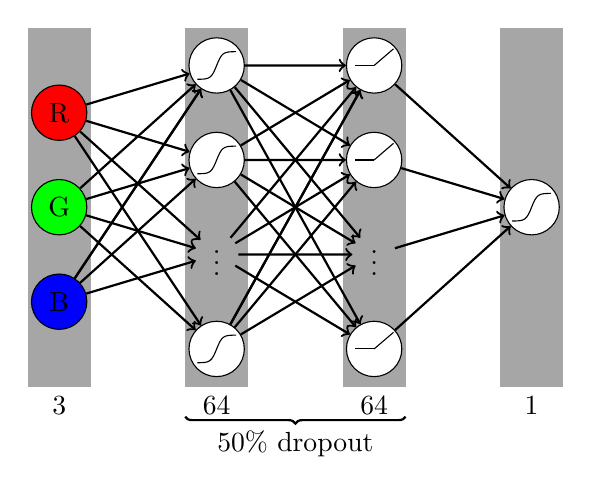
\begin{tikzpicture}[scale=2,yscale=0.6]
    \fill[layer] (  -\width,-1.9) rectangle (  \width,1.9);
    \fill[layer] (1+-\width,-1.9) rectangle (1+\width,1.9);
    \fill[layer] (2+-\width,-1.9) rectangle (2+\width,1.9);
    \fill[layer] (3+-\width,-1.9) rectangle (3+\width,1.9);
    \node (l1label) at  (0, -2.1) {3};
    \node (l2label) at  (1, -2.1) {64};
    \node (l3label) at  (2, -2.1) {64};
    \node (l4label) at  (3, -2.1) {1};
    \node (r)[input,fill=red]   at (0, 1) {R};
    \node (g)[input,fill=green] at (0, 0) {G};
    \node (b)[input,fill=blue]  at (0,-1) {B};

    \node (h11)[hidden, sigmoid] at (1, 1.5) {};
    \node (h12)[hidden, sigmoid] at (1, 0.5) {};
    \node[circle, inner sep=0] (h13) at (1,-0.5) {\vdots};
    \node (h14)[hidden, sigmoid] at (1,-1.5) {};
    \node (h21)[hidden, relu] at (2, 1.5) {};
    \node (h22)[hidden, relu] at (2, 0.5) {};
    \node[circle, inner sep=0] (h23) at (2,-0.5) {\vdots};
    \node (h24)[hidden, relu] at (2,-1.5) {};

    \node (o1)[output, sigmoid] at (3,0) {};

    \draw[stateTransition] (r) -- (h11) node [midway,above=-0.06cm] {};
    \draw[stateTransition] (r) -- (h12) node [midway,above=-0.06cm] {};
    \draw[stateTransition] (r) -- (h13) node [midway,above=-0.06cm] {};
    \draw[stateTransition] (r) -- (h14) node [midway,above=-0.06cm] {};
    \draw[stateTransition] (g) -- (h11) node [midway,above=-0.06cm] {};
    \draw[stateTransition] (g) -- (h12) node [midway,above=-0.06cm] {};
    \draw[stateTransition] (g) -- (h13) node [midway,above=-0.06cm] {};
    \draw[stateTransition] (g) -- (h14) node [midway,above=-0.06cm] {};
    \draw[stateTransition] (b) -- (h11) node [midway,above=-0.06cm] {};
    \draw[stateTransition] (b) -- (h12) node [midway,above=-0.06cm] {};
    \draw[stateTransition] (b) -- (h13) node [midway,above=-0.06cm] {};
    \draw[stateTransition] (b) -- (h11) node [midway,above=-0.06cm] {};

    \draw[stateTransition] (h11) -- (h21) node [midway,above=-0.06cm] {};
    \draw[stateTransition] (h11) -- (h22) node [midway,above=-0.06cm] {};
    \draw[stateTransition] (h11) -- (h23) node [midway,above=-0.06cm] {};
    \draw[stateTransition] (h11) -- (h24) node [midway,above=-0.06cm] {};
    \draw[stateTransition] (h12) -- (h21) node [midway,above=-0.06cm] {};
    \draw[stateTransition] (h12) -- (h22) node [midway,above=-0.06cm] {};
    \draw[stateTransition] (h12) -- (h23) node [midway,above=-0.06cm] {};
    \draw[stateTransition] (h12) -- (h24) node [midway,above=-0.06cm] {};
    \draw[stateTransition] (h13) -- (h21) node [midway,above=-0.06cm] {};
    \draw[stateTransition] (h13) -- (h22) node [midway,above=-0.06cm] {};
    \draw[stateTransition] (h13) -- (h23) node [midway,above=-0.06cm] {};
    \draw[stateTransition] (h13) -- (h24) node [midway,above=-0.06cm] {};
    \draw[stateTransition] (h14) -- (h21) node [midway,above=-0.06cm] {};
    \draw[stateTransition] (h14) -- (h22) node [midway,above=-0.06cm] {};
    \draw[stateTransition] (h14) -- (h23) node [midway,above=-0.06cm] {};
    \draw[stateTransition] (h14) -- (h21) node [midway,above=-0.06cm] {};

    \draw[stateTransition] (h21) -- (o1) node [midway,above=-0.06cm] {};
    \draw[stateTransition] (h22) -- (o1) node [midway,above=-0.10cm] {};
    \draw[stateTransition] (h23) -- (o1) node [midway,above=-0.06cm] {};
    \draw[stateTransition] (h24) -- (o1) node [midway,above=-0.06cm] {};

    \draw [
    thick,
    decoration={
        brace,
        mirror,
        raise=0.5cm
    },
    decorate
] (1+-\width, -1.8) -- (2+\width, -1.8)
node [pos=0.5,anchor=north,yshift=-0.55cm] {50\% dropout};
\end{tikzpicture}
    \caption{Architecture of the baseline model.}
    \label{fig:baseline-architecture}
\end{figure}
